\documentclass[10pt]{standalone}
\usepackage{tikz}

% TikZ libraries `calc` needed now to tweak bracket.
\usetikzlibrary{backgrounds,fit,decorations.pathreplacing,calc}
% Dirac Kets
\newcommand{\ketone}[1]{\ensuremath{\left|#1\right\rangle^{\otimes nd}}}

\newcommand{\kettwo}[1]{\ensuremath{\left|#1\right\rangle^{\otimes n_0}}}

\newcommand{\ket}[1]{\ensuremath{\left|#1\right\rangle}}

\begin{document}
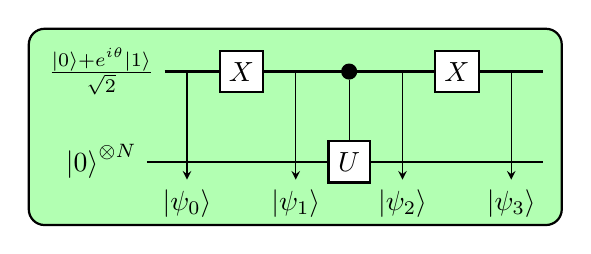
\begin{tikzpicture}[thick]
	% `phase' is used for controlled phase gates (dots).
	% `surround' is used for the background box.
	\tikzstyle{operator} = [draw,fill=white,minimum size=1.5em] 
	\tikzstyle{phase} = [draw,fill,shape=circle,minimum size=5pt,inner sep=0pt]
	\tikzstyle{surround} = [fill=green!30,thick,draw=black,rounded corners=2mm]
	%
	\matrix[row sep=0.4cm, column sep=0.4cm] (circuit) {
	% First row.
		\node (q10) {$\frac{\ket 0 + e^{i\theta}\ket 1}{\sqrt 2}$}; &[-0.5cm]
		&
		\coordinate (q11);&
		\node[operator] (q12) {\ensuremath{X}}; &
		\coordinate (q13);&
		\node[phase] (q14) {};&	
		\coordinate (q15);&
		\node[operator] (q16) {\ensuremath{X}}; &
		\coordinate (q17);&
		\coordinate (end1); \\
	
		% Second row.
		\node (q20) {$\ket{0}^{\otimes N}$}; &
		&
		\coordinate (q21);&
		\coordinate (q22);& 
		\coordinate (q23);&
		\node[operator] (q24) {\ensuremath{U}}; & 
		\coordinate (q25);&
		\coordinate (q26);& 
		\coordinate (q27);&
		\coordinate (end2);\\
		};
	% Draw bracket on right with resultant state.
		%\node[rectangle, draw, fill=white, minimum width = 1.5em, minimum height = 1.65cm][fit = (q17) (q27)] (box) {};
		%\node[align=center] at (box.center){A};
	\begin{pgfonlayer}{background}
		% Draw background box.
		\node at([yshift=-1.6em]end2) (corner) {};
		\node[surround] (background) [fit = (q10) (corner)] {};
		% Draw lines.
		\draw[thick] (q10) -- (end1)  (q20) -- (end2) ;
		\node at ([yshift=-1.5em]q21) (psi0) {\ket{\ensuremath{\psi_0}}};
		\draw[->, >=stealth] (q11) -- (psi0);
		\node at ([yshift=-1.5em]q23) (psi1) {\ket{\ensuremath{\psi_1}}};
		\draw[->, >=stealth] (q13) -- (psi1);
		\node at ([yshift=-1.5em]q25) (psi2) {\ket{\ensuremath{\psi_2}}};
		\draw[->, >=stealth] (q15) -- (psi2);
		\node at ([yshift=-1.5em]q27) (psi3) {\ket{\ensuremath{\psi_3}}};
		\draw[->, >=stealth] (q17) -- (psi3);
		\draw (q14) -- (q24);
		%\node at ([yshift=-1.5em]q210) (psi4) {\ket{\ensuremath{\psi_4}}};
		%\draw[->, >=stealth] (q111) -- (psi4);
	\end{pgfonlayer}
%
\end{tikzpicture}
\end{document}
